% Diese Zeile bitte -nicht- aendern.
\documentclass[course=erap]{aspdoc}
\graphicspath{ {./images/} }
%%%%%%%%%%%%%%%%%%%%%%%%%%%%%%%%%
%% TODO: Ersetzen Sie in den folgenden Zeilen die entsprechenden -Texte-
%% mit den richtigen Werten.
\newcommand{\theGroup}{142} % Beispiel: 42
\newcommand{\theNumber}{A213} % Beispiel: A123
\author{Anton Baumann \and Felix Brandis \and Michal Cizevskij}
\date{Sommersemester 2020} % Beispiel: Wintersemester 2019/20
%%%%%%%%%%%%%%%%%%%%%%%%%%%%%%%%%

% Diese Zeile bitte -nicht- aendern.
\title{Gruppe \theGroup{} -- Abgabe zu Aufgabe \theNumber}

\begin{document}
\maketitle

\section{Einleitung}

Um die in der Vorlesung erlangten Kenntnisse zu vertiefen, wird vom Lehrstuhl für Rechnerarchitektur und Parallele Systeme ein Semester begleitendes Praktikum angeboten.\\
Im Rahmen diesen Rechnerarchitektur Praktikums hat sich unsere Gruppe mit dem Thema der Moore Kurve auseinandergesetzt. Die Moore Kurve ist eine von dem Mathematiker Eliakim Hastings Moore (1862-1932) entwickelte raumfüllende Kurve. Sie basiert auf der Hilbert Kurve und findet oft Anwendung in Bildverarbeitung und Datendarstellung. Unsere erste Aufgabe war es einen Algorithmus in Assembler zu entwickeln der die Moore Kurve beliebigen Grades erstellt und in einer Datei abbildet. Die zweite Aufgabe war es zu beantworten, ob es möglich ist einen beliebigen Punkt der Kurve in konstanter Zeit unabhängig vom Grad zu berechnen.\\
\\
\begin{center}
	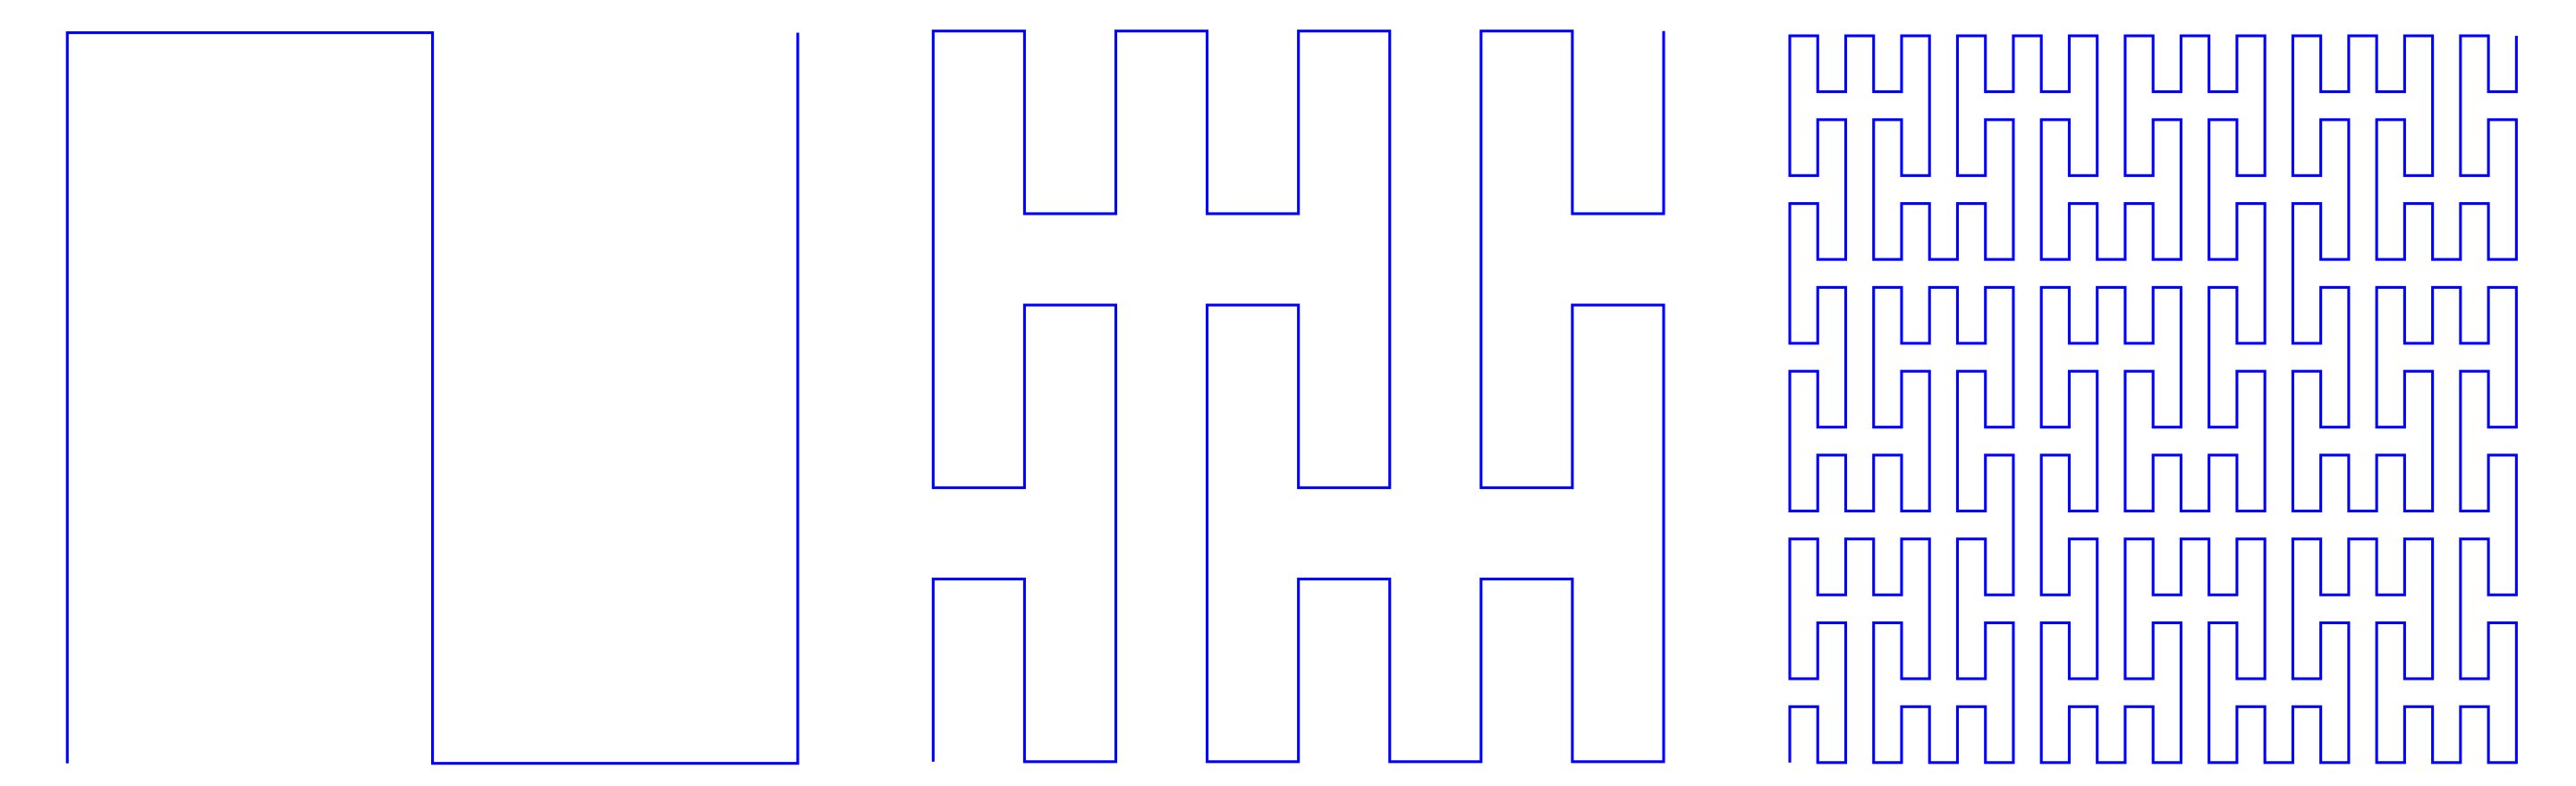
\includegraphics[width=12cm, height=4cm]{Peano}\\ %cite
	\tiny Figur 1: Die drei ersten Iterationen der Peano Kurve
\end{center}
\	\\
Generell ist eine raumfüllenden Kurve (Englisch: space-filling curve oder auch SFC) eine "Linie" die von einem Eindimensionalen Raum auf ein N-Dimensionalen Raum abbildet. einfachheitshalber beschränken wir uns aber auf zweidimensionalen und ein Beispiel im dreidimensionalen Raum. Die Besonderheit dieser Kurve liegt darin, dass sie jeden Punkt des Einheitsquadrats passiert. Genauer gesagt, wenn n für den Grad der Kurve steht und $\lim_{n\to\infty}$, dann wird eine gegebene Fläche durch so eine Kurve gefüllt.\\
Die erste SFC wurde von einem Italienischen Mathematiker Giuseppe Peano in 1890 entwickelt. 
\newpage
Die Motivation für solch eine Erkenntnis bekam er durch einen weitern  renommierten Mathematiker Georg Cantor der wenige Jahre zuvor bewiesen hatte, dass die Mengen der Natürlichen zahlen und die der positiven rationalen Zahlen gleich mächtig sind (Cantors erstes diagonal Argument). 
Durch das verallgemeinern des Cantorischen Diagonalarguments kann man zeigen, dass es eindimensionale Objekte gibt, die zweidimensionale füllen können. Eine raumfüllende Kurve ist also eine surjektive Abbildung, die von einem Einheitsintervall in ein Einheitsquadrat abbildet.
\\
\\
\begin{center}
	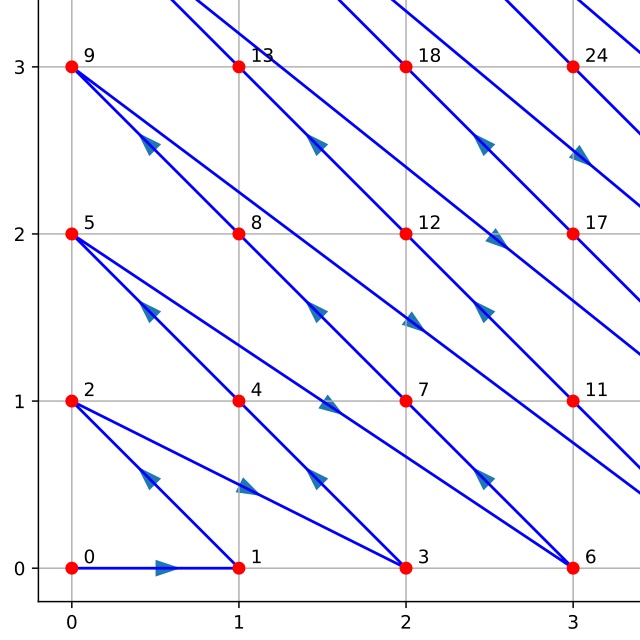
\includegraphics[width=5cm, height=5cm]{Cantor}\\	%cite
	\tiny Figur 2: Cantorische Paarungsfunktion
\end{center}
\	\\
\\
Die Hilbert Kurve, die von dem gleichnamigen Mathematiker David Hilbert in 1891 entwickelt wurde ist eine einfachere Version die das Einheitsquadrat in 4 Teile anstatt 9 partitioniert. Diese Quadranten beinhalten dann die Hilbert Kurve vom Grad n - 1. Betrachtet man zum Beispiel die mittlere Abbildung in Fig. 3 ,entsprechend Hilbert von Grad 2. Dann bemerkt man, dass sie vier mal die Kurve vom Grad 1 beinhaltet, die rotiert oder gespiegelt wurde und an den End- bzw. Startpunkten verbunden wurden.
\\
\\
\begin{center}
	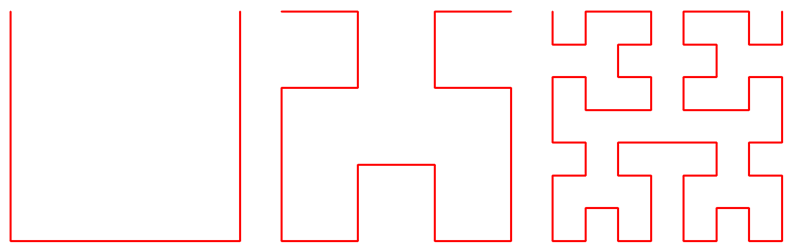
\includegraphics[width=12cm, height=4cm]{Hilbert}\\	%cite
	\tiny Figur 3: Die drei ersten Iterationen der Hilbert Kurve
\end{center}
\	\\
\newpage %Autor der Moore Kurve ist im Abstract erwähnt fehlt datum leider
Wie bereits erwähnt ist die Moore Kurve eine Variation der Hilbert Kurve. Die ersten Grade der Moore- und Hilbert-Kurve sind äquivalent. Dabei ergeben sich die weiteren Iterationen der Moore Kurve, durch die Zusammensetzung der Hilbert Kurve vom Grad n - 1.  Also bis zum Grad n -1 zeichnet man eine Hilbert Kurve, jedoch beim Grad n ordnet man die 4 Hilbert Kurven vom Grad n - 1 anders an.\\ % wie genau ist dann Lösungsweg
Bemerkenswert ist, dass im Gegensatz zur Hilbert Kurve, die Moore Kurve so konstruiert ist, sodass der Anfangspunkt und Endpunkt sich nebeneinander befinden.
\\
\\
\begin{center}
	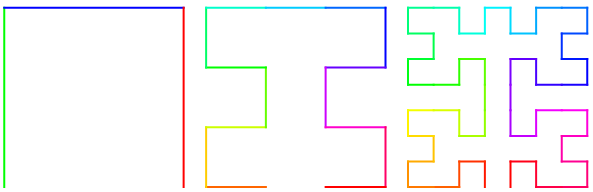
\includegraphics[width=12cm, height=4cm]{Moore}\\	%cite
	\tiny Figur 4: Die drei ersten Iterationen der Moore Kurve
\end{center}
\	\\
Außerdem gehört die Moore Kurve (Peano und Hilbert ebenfalls) einer Unterkategorie der SFC die man FASS Kurven nennt. (FASS: „space-filling, self-avoiding, simple and self-similar“).\\
Dies birgt wichtige Eigenschaften weshalb sie in der Praxis Verwendung findet. Zu einem die Kurve ist selbst ausweichend, das bedeutet jeder Punkt ist exakt festgelegt/bestimmt, also wird nur einmal durchlaufen. Hinzu behält die Kurve die Lokalität der Punkte bei. Das bedeutet, sind die Punkte nah beinander im eindimensionalen Einheitsintervall, so sind sie es ebenfalls in der Kurve. % http://blog.christianperone.com/2015/08/googles-s2-geometry-on-the-sphere-cells-and-hilbert-curve/
\\
\\
\begin{center}
	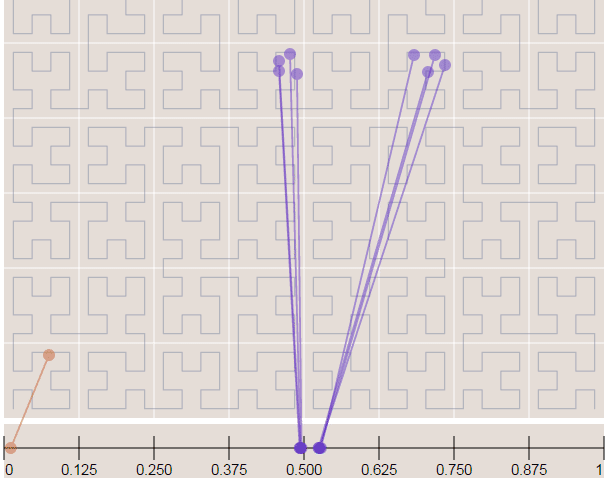
\includegraphics[width=8cm, height=6cm]{Locality}\\	%cite
	\tiny Figur 5: Graphik um die Eigenschaft der Lokalität zu verdeutlichen % for spatial DB = raumbezogene Datenbank
\end{center} %Since S2 uses the Hilbert Curve to enumerate the cells								% UMFOLMOLIERUNG MORGEN
\newpage %It’s a quadtree projected onto the unit sphere, plus using the Hilbert curve for a fast mapping between integer indices and cells. Hilbert curve is a space-filling curve that converts multiple dimensions into one dimension that has an special spatial feature: it preserves the locality.
Ein Beispiel der Verwendung einer raumfüllenden Kurve ist bei der raumbezogenen Indexierung von geographischen Daten. Sehr einfach ausgedrückt funktioniert es Folgend: man unterteilt (in unserem Fall die Erde) sein Gebiet in viereckige Zellen. Diese dienen der kompakten Darstellung einer bestimmten Region. Um. diese Zellen schell "ansprechen" zu können indexieren wir sie. Dabei ist es uns wichtig, dass wenn sie geographisch nah beinander liegen, dass  sie dies auch im Feld tun. Da eine FASS Kurve genau diese Anforderungen erfüllt eignet sie sich für solch eine Verwendung. Ein konkretes Beispiel der Anwendung wäre die \href{https://code.google.com/archive/p/s2-geometry-library/}{S2-geometry-library von Google}. 
% vielleicht noch erwähnen das es alternativen gibt aber zb Hilbert kurve sehr effizient ist
\\
\begin{center}
	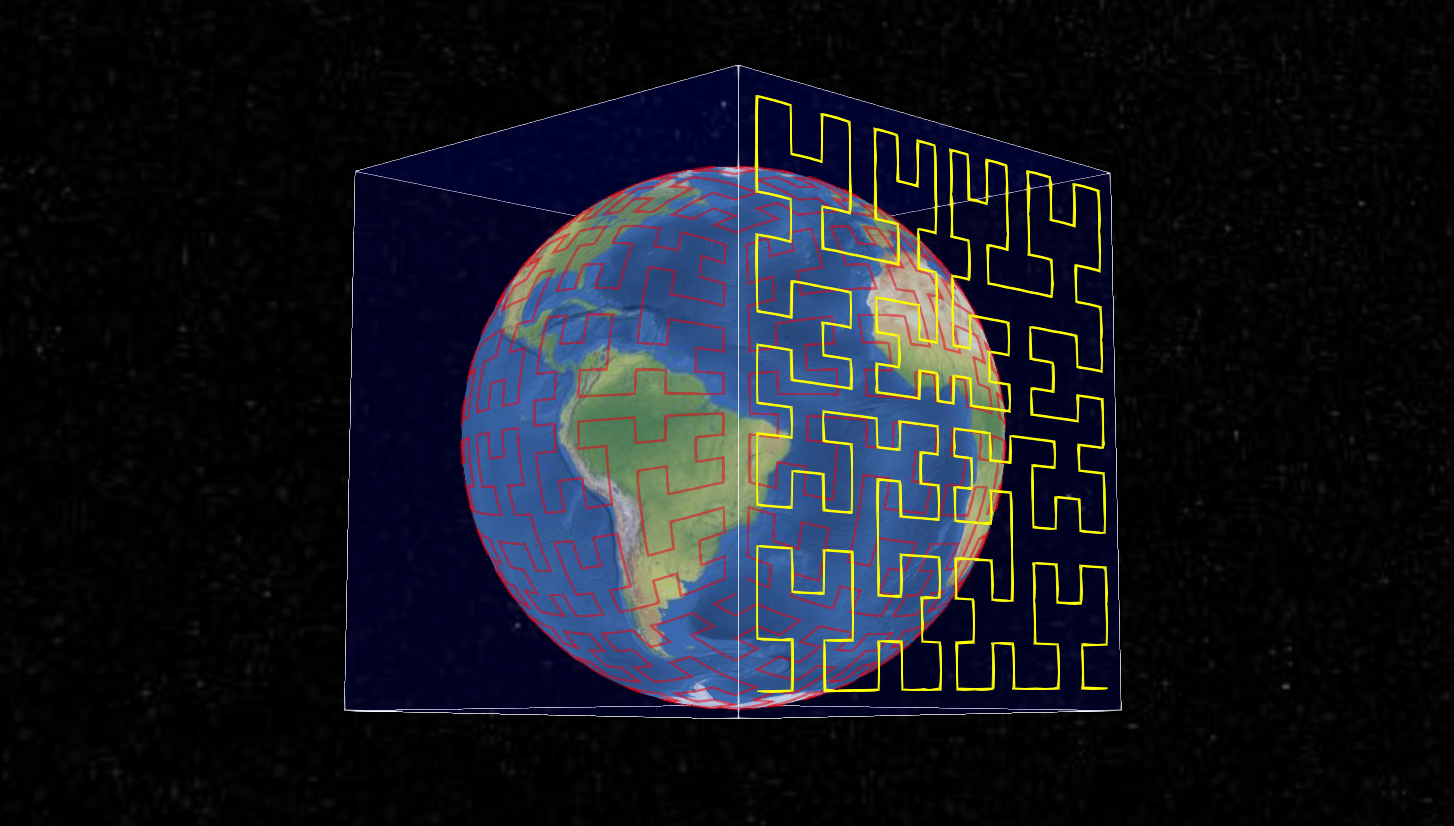
\includegraphics[width=9cm, height=6cm]{Earth}\\	%cite
	\tiny Abbildung 6: Einteinlung der Erde %https://medium.com/sidewalk-talk/s2-cells-and-space-filling-curves-keys-to-building-better-digital-map-tools-for-cities-a312aa5e2f59
\end{center}


\section{Lösungsansatz}


% TODO: Je nach Aufgabenstellung einen der Begriffe wählen
\section{Korrektheit/Genauigkeit}


\section{Performanzanalyse}


\section{Zusammenfassung und Ausblick}

% TODO: Fuegen Sie Ihre Quellen der Datei Ausarbeitung.bib hinzu
% Referenzieren Sie diese dann mit \cite{}.
% Beispiel: CR2 ist ein Register der x86-Architektur~\cite{intel2017man}.
\bibliographystyle{plain}
\bibliography{Ausarbeitung}{}

\end{document}
